\documentclass[]{article}
\usepackage[UTF8]{ctex}
\usepackage[a4paper,left=10mm,right=10mm,bottom=10mm,top=10mm]{geometry}
\usepackage{graphicx}
\usepackage{float}
\usepackage{amsmath,amsfonts,amssymb,amsthm}
\usepackage{array,color}
%opening
\title{计算机科学中的数学基础Exercise11}
\author{陈昱衡 521021910939}
\date{\today}

\begin{document}

\maketitle



\section*{Warmups7}
\begin{figure}[H]
	
\includegraphics[scale=1]{Q1.png}
\end{figure}
若第一个被删除的人是10号,那么m满足
\begin{equation}
m \bmod 10  = 0
\end{equation}
若紧接着第二个被删除时人是k,
那么由于有十个人,而第一次删除的恰好是10号,那么第二轮相当于有九个人,从头开始删除,
那么m满足
\begin{equation}
	m \bmod 9 = k
\end{equation}
若紧接着删除编号为$k+1$的人,那么m满足
\begin{equation}
	m \bmod 8 = 1
\end{equation}
而$m$若同时满足这些条件,就有$m$既为奇数,又为偶数,故不存在这样的$m$。
\section*{Warmups8}
\begin{figure}[H]
%	\centering
	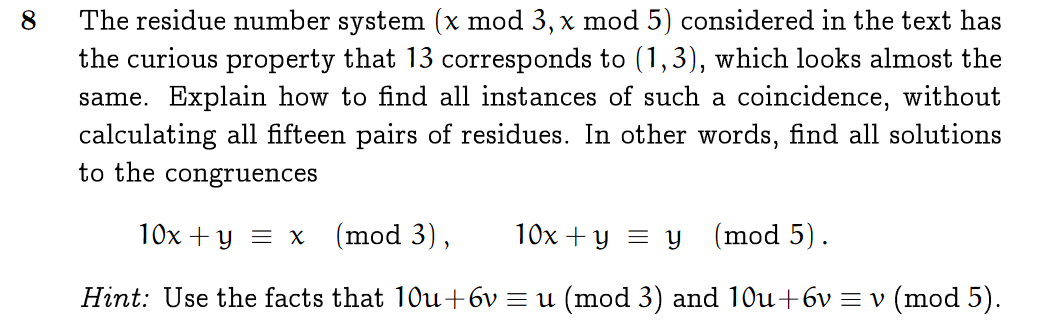
\includegraphics[scale=1]{Q2}
%	\caption{}
%	\label{fig:q2}
\end{figure}
根据题意,$x,y$满足,
\begin{align}
	10x+y &\equiv x \bmod 3\\
	10x+y &\equiv y \bmod 5
\end{align}
根据提示,
\begin{align}
	10x + 6y &\equiv x \bmod 3\\
	10x + 6y &\equiv y \bmod 5
\end{align}
所以,两式相减,有
\begin{align}
	5y&\equiv0 \bmod 5\\
\end{align}
得到, $y=0$或$y=3$
代入,可得
$x=0$或$x=1$.
\section*{Warmups9}
\begin{figure}[H]
	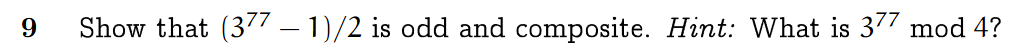
\includegraphics[scale = 1]{Q3}
\end{figure}
由二项式展开,
有
\begin{align}
	3^{77}-1&=(4-1)^{77}-1\\
	&=4^{77} - 77 \times 4^{76} + \cdots + 77 \times 4 - 4 + 3 \\
\end{align}
故,根据提示,可以计算得,
\begin{equation}
	3^{77} -1 \bmod 4 = 3
\end{equation}
故,可以计算得到,$\frac{3^{77}-1}{2}$是奇数。
同时,由等差数列求和公式,
\begin{align}
	\frac{3^{77}-1}{2} &= 1 + 3+ 3^2 + 3*3 +\cdots + 3^{77}\\
	&= (1+3+3^2 + \cdots + 3^7) + 3^8 \times (1+3+3^2 + \cdots + 3^7) + \cdots + 3^{70} \times (1+3+3^2 + \cdots + 3^7)\\
	& = (1+3+3^2 + \cdots + 3^7) \times (1 + 3^8 + \cdots + 3^{70})
\end{align}
故,$\frac{3^{77}-1}{2}$是奇的合数。

\section*{Basics17}
\begin{figure}[H]
	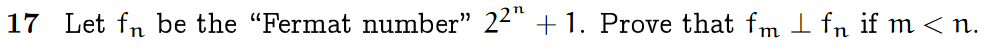
\includegraphics[scale = 1]{Q4}
\end{figure}
观察费马数,猜测,
\begin{equation}
	f_{n} = f_{n-1} \times f_{n-2} \times f_{0} + 2
\end{equation}
现用数学归纳法证明。
易证,当$n=1$时,有
\begin{equation}
	f_{1} = 5 = 4 + 1 = 3 +2=f_{0} + 2
\end{equation}
假设,当第$n-1$项满足时,有
\begin{align}
	f_{n} &= 2^{2^n} + 1\\
	f_{n-1} &= 2^{2^{n-1}} + 1 \\
	&=f_{n-2} \times f_{0} + 2\\
	f_{n-2} \times \cdots f_{0} &= 2^{2^{n-1}} -1 \\
	f_{n-1} \times f_{n-2} \times \cdots \times f_{0} &= (2^{2^{n-1}} -1)\times (2^{2^{n-1}}+1)\\
	&=2^{2^{n}} - 1\\
	&=f_{n} - 2
\end{align}
故,
\begin{equation}
	f_{n} = f_{0} \times f_{1} \times \cdots \times f_{n-1} + 2
\end{equation}

故,因为$m \le n$
\begin{equation}
	f_{n} \bmod f_{m} \equiv 2
\end{equation}
由
\begin{equation}
	gcd(n,  m) =gcd (n \bmod m, m)
\end{equation}
得,
\begin{align}
	gcd(f_{n},f_{m}) &= gcd (f_{n} \bmod f_{m}, f_{m}) \\
	&=gcd (2,f_{m})\\
	&=1
\end{align}
故,得到$f_{m}$和$f_{m}$互素。
\end{document}